\chapter{Gambar dan Laporan Kinerja Tambahan N=4}
\label{appendix:additional_results_n4}

Bagian ini menyajikan visualisasi tambahan mengenai arsitektur sirkuit kuantum, analisis pengaruh kedalaman sirkuit, serta laporan ringkasan kinerja portofolio untuk sistem dengan $N=4$ aset.

\section{Arsitektur Sirkuit Kuantum N=4}
\label{appendix:circuit_diagram_n4}

\begin{figure}[H]
    \centering
    
\includegraphics[width=0.9\textwidth]{GTQuantumInvest/Hasil_N4_GT/rangkaian_kuantum_depth3_N4.png}
    \caption{Rangkaian Sirkuit Kuantum N=4 dengan Kedalaman (\textit{Depth}) 3}
    \label{fig:circuit_diagram_n4}
\end{figure}

\section{Analisis Kedalaman Sirkuit N=4 (\textit{Depth Analysis})}
\label{appendix:depth_analysis_n4}

\begin{figure}[H]
    \centering
    
\includegraphics[width=0.8\textwidth]{GTQuantumInvest/Hasil_N4_GT/grafik_depth_per_window_N4.png}
    \caption{Grafik Performa Energi Hamiltonian N=4 terhadap Variasi \textit{Depth}}
    \label{fig:depth_energy_plot_n4}
\end{figure}

\section{Ringkasan Kinerja Strategi N=4 (\textit{Backtest Report})}
\label{appendix:backtest_report_n4}

\begin{figure}[H]
    \centering
    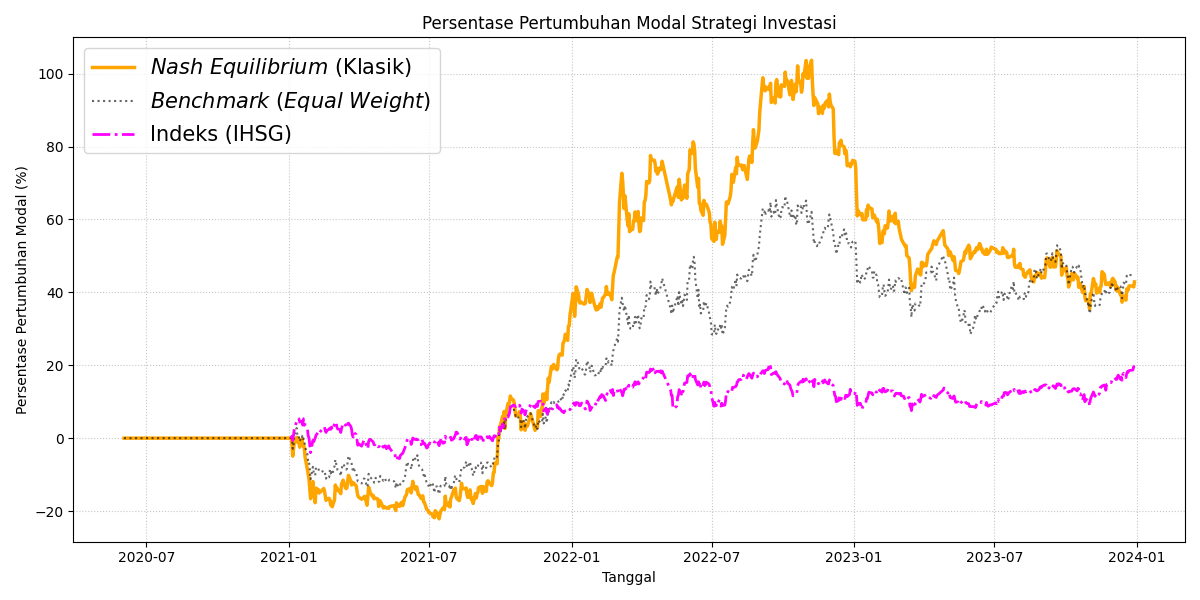
\includegraphics[width=0.85\textwidth]{GTQuantumInvest/Hasil_N4_GT/hasil_backtest_nash_N4.png}
    \caption{Kurva Performa Kumulatif (\textit{Backtesting}) Strategi \textit{Nash Equilibrium} (Klasik) N=4}
    \label{fig:backtest_curve_nash_n4}
\end{figure}

\begin{figure}[H]
    \centering
    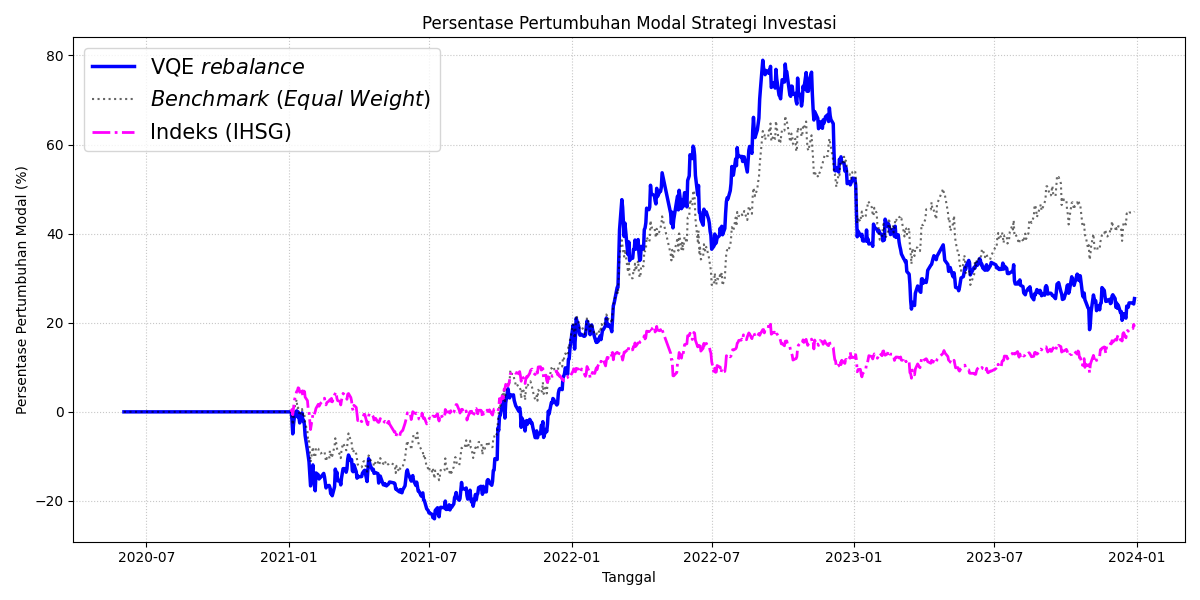
\includegraphics[width=0.85\textwidth]{GTQuantumInvest/Hasil_N4_NoGT/hasil_backtest_vqe_N4.png}
    \caption{Kurva Performa Kumulatif (\textit{Backtesting}) Strategi \textit{Quantum VQE} (Tanpa \textit{Warm-Start}) N=4}
    \label{fig:backtest_curve_vqe_nogt_n4}
\end{figure}

\begin{figure}[H]
    \centering
    
\includegraphics[width=0.85\textwidth]{GTQuantumInvest/Hasil_N4_GT/hasil_backtest_vqe_N4.png}
    \caption{Kurva Performa Kumulatif (\textit{Backtesting}) Strategi \textit{Quantum VQE} (Dengan \textit{Warm-Start} GT) N=4}
    \label{fig:backtest_curve_vqe_gt_n4}
\end{figure}
